\begin{frame}

\Huge{\centerline{TRANSLATOR}}
\end{frame}

\begin{frame}
\frametitle{Aim of Translator Service}
\begin{figure}
\centering
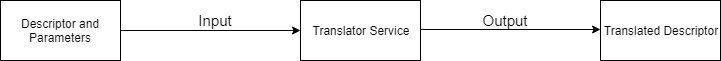
\includegraphics[width=1\linewidth]{images/img-1-translate}
\label{Figure1}
\end{figure}
Translator receives as input descriptor files to be translated and parameters, such as ``Osm-to-Sonata" if OSM descriptor has to be translated to Sonata or ``Sonata-to-osm" if Sonata descriptor has to be translated to OSM. The output of the translator is a translated descriptor as per the parameter 
\end{frame}

\begin{frame}
\frametitle{Working of Translator Service}
\begin{figure}
\centering
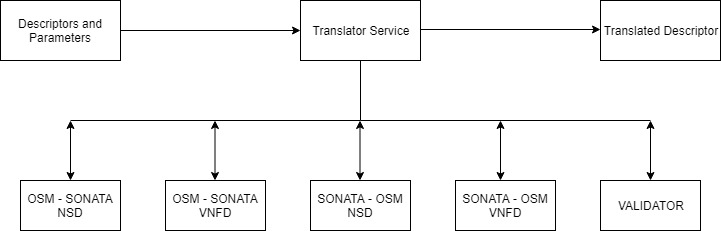
\includegraphics[width=1\linewidth]{images/img-2-translate}
\label{Figure2}
\caption{processing of descriptor file within translator}
\end{figure}
\end{frame}

\begin{frame}
\frametitle{Milestone and challenges}
\textbf{Milestone}:\\
\begin{itemize}
\item The translator can successfully translate simple NSD and VNFD descriptors and validate them.
\end{itemize}

\textbf{Challenges}:\\
\begin{itemize}
\item Translation: have  to work on additional properties such as "monitoring parameters", "forwarding graphs".
\item Validation: Issue with OSM descriptor validation
\end{itemize}

\end{frame}